\documentclass[12pt,fleqn]{article}\usepackage{../common}
\begin{document}
Felzenswalb Gruplamasi (Felzenswalb Clustering)

Minimum Kapsayan Agac (Minimum Spanning Tree -MST-) kavramini kullanan
Felzenswalb kumelemesini gorecegiz. MST'yi daha once isledik. Literaturde
Felzenswalb metotunun imaj gruplamasi icin kullanildigini gorebilirsiniz,
biz imaj gruplamasi yapan algoritma icinden veri kumelemesi yapan kismi
cikarttik ve ayri bir sekilde paylasiyoruz. Bu gruplama algoritmasinin daha
once paylastigimiz Kruskal'in MST koduna yapilacak birkac ekleme sayesinde
elde edilebilmesi hakikaten ilginc. Normal MST cizitin ayri bolgelerinde
ayri agaclar yaratir ve bunlari yavas yavas buyutur, gerektigi noktalarda
onlari birlestirir. Felzenswalb sadece bu birlestirme mantigini biraz
degistirip, ayri agaclari bir grup olarak kabul eder, ve bu gruplarin kendi
icinde benzerligin maksimal gruplararasi benzerligin minimal olacak hale
getirir. Bu sekilde bildik Kruskal isletilince cok hizli isleyen hizli bir
gruplama algoritmasi elde edilmis olur!

Felzenswalb veri olarak, MST gibi, bir cizit alir, bu cizit veri
noktalarinin arasindaki yakinlik bilgisini iceren bir matris olarak
verilebilir. Mesela 5 veri noktasi var ise, 0. nokta ile 1. nokta
arasindaki '10' buyuklugundeki bir mesafe $A(0,1) = 10$ olarak
kaydedilebilir. Kumeler birbirine yakin ogeler arasindan secilir.

Algoritmanin onemli avantajlarindan biri kume sayisinin (KMeans'de oldugu
gibi) onceden tanimlanmasina gerek olmamasidir. Belli esik degerleri
tanimlaninca kume sayisi kendiliginden bulunur. Tabii ``disaridan verilen
bir parametreyi baska biriyle degistirmis mi olduk?'' sorusu akla
gelebilir, Felzenswalb'in aldigi hiperparametreler kabaca ayarlanabilen ve
veri kaynagi baglaminda akla uygun seyler, ve belli degerler etrafinda
stabilite ortaya cikabiliyor. Kiyasla ``kume sayisi'' ciddi bir rakam ve
degismesi mumkun degil. 

Felzenswalb'in matematiginde once imaj bolgelerinin (ya da veri kumeleri
olarak dusunebiliriz) ikili karsilastirmaya bir olcut gerekir. Bu bolumde
bir beyan $D$'yi ortaya koyacagiz, ki bu beyan, imajdaki iki bilesen (ki
imaj gruplamasinin dogru olarak bulmaya calisacagi bilesenler) arasinda bir
sinir olup olmadigina dair kanitin olcusu olacak. Beyanin temeli sudur: iki
bilesen arasindaki sinirin boyunda yer alan her iki tarafin ogelerinin
farkliligina bak, ve onu her bilesenin kendi icindeki farkliliga gore
oranla. Yani bu beyan, bir bilesenin ic farkliligini dis farkliligina
kiyaslar, ve bu sebeple verinin yerel karakteristikleri gozetmis
olur. Kiyaslama mesela, global, verinin her yerinde aynen gecerli olacak
bir sabit esik degerine vs. bagli degildir.

Tanim

Bir bilesen $C \subseteq V$, ki $C$ bir bilesendir (component) ve $V$ cizitin tum
noktalaridir, {\em ic farkliligini}, o $C$'nin minimum kapsayan agacinin,
yani $MST(C)$'sinin en buyuk kenar agirligi olarak aliyoruz. Bu ic farkliligi
$Int(C)$ olarak belirtirsek, 

$$ Int(C) = \max_{e \in MST(C,E)} w(e) $$

ki $w((v_i , v_j))$ bir cizit $G = (V,E)$'yi olusturan bir kenar $(v_i,v_j)
\in E$ agirligi 
olarak belirtilir. 

Tanim

Iki bilesen $C_1,C_2 \subseteq V$ arasindaki farki o iki bileseni
birlestiren kenarlardan en ufagi olarak aliyoruz. Iki bilesenin arasinda
birden fazla baglanti olmasi mumkundur, tum bunlara bakiyoruz, ve en
ufagini aliyoruz.

$$ Dif(C_1,C_2) = \min_{v_i \in C_1, v_j \in C_2, (v_i,v_j) \in E} w((v_i,v_j))$$

Eger $C_1,C_2$ arasinda bir kenar yok ise $Dif(C_1,C_2) = \infty$ kabul
ediliyor. 

Prensip olarak iki bilesen arasindaki en minimal baglantinin problem
cikartabilecegi dusunulebilirdi, niye en az, niye ortalama vs degil? Fakat
pratikte bu olcutun cok iyi isledigini gorduk. Hatta iyi olmaktan ote, bu
olcutu minimal yerine medyan, ya da diger ceyreksel (quantile) olcute
degistirdigimiz zaman (ki bunu yaparak aykiri degerlere -outlier- karsi
daha dayanikli olmasini istemistik), algoritma cetrefilligi NP-Zor haline
geliyor. Yani gruplama kriterinde ufacik bir degisiklik problemin cozum
zorlulugunda muthis bir degisim ortaya cikartiyor. 

Simdi iki bilesenin karsilastirma beyani $D$'nin tanimina geldik. $D$ olcutu,
$Dif(C_1,C_2)$'nin $Int(C_1)$ ya da $Int(C_2)$'den herhangi birinden daha
buyuk olup olmadigina bakar. Ayrica bu karsilastirmayi bir esik degeri
uzerinden pay ekleyerek yapar, eger irdeleme olumlu ise, iki bilesen
arasinda sinir vardir, yoksa yoktur.

$$ 
D(C_1,C_2) = 
\left\{ \begin{array}{ll}
Dogru & \textrm{ Eger } Dif(C_1,C_2) > MInt(C_1,C_2) \textrm{ ise } \\
Yanlis & \textrm{ Diger durumda }
\end{array} \right.
 $$

Minimum ic fark $MInt$ ise soyle tanimlidir,

$$ 
MInt(C_1,C_2) = \min (Int(C_1)+\tau(C_1), Int(C_2)+\tau(C_2))
 $$

Esik fonksiyonu $\tau$ ustteki irdeledigimiz fark hesaplarinin belli
derecelerde disaridan etkilemek icin koyulmustur. Eger bunu kullanmasaydik
sadece $Int$ fonksiyonunu kullanmamiz gerekecekti, fakat bu olcut tek
basina ufak bir bilesenin yerel karakteristiklerini gostermesi acisindan yeterli
degildir. Asiri durumda mesela $|C| = 1,Int(C)=0$, yani en kucuk $C$
durumudur bu ($|C|$ bilesenin icindeki oge sayisi), icinde tek oge vardir,
ve hicbir kenar yoktur, $Int(C) = 0$.  

Bu sebeple iyi bir $\tau$ bilesenin buyuklugunu hesaba katarak, ona ters
oranli bir rakam olusturursa iyi olur, mesela bir sabit $k$ uzerinden,

$$ \tau(C) = \frac{k}{|C|} $$

Bu demektir ki ufak bilesenler icin daha kuvvetli bir ispat ariyoruz, cunku
kucuk $|C|$, $\tau$'yu buyutecektir, ve $Dif$'in ondan buyuk olmasi daha
zorlasacaktir. Tabii dikkat edelim, $k$ bir ``bilesen sayisi'' degildir,
yani fonksiyonuna dikkatli bakarsak, eger bilesenler arasinda yeterince
buyuk bir fark var ise ufak bilesenlere hala izin verilmistir.

Algoritma soyledir, girdi olarak $G=(V,E)$ alir, ve $V$'yi $S$
bilesenlerine ayirir ki her $S$ icinde ona ait olan kenarlar vardir, yani
$S=(C_1,..,C_r)$ 

\begin{algorithm}[h]
\begin{pseudocode}
\codename $\code{felzenswalb}\left(G\right)$\\
\codeline \> $E$ kenarlarini $\pi = (o_1,..,o_m)$ seklinde kucukten buyuge dogru sirala. \\
\codeline \> Ilk basta $S^0$ gruplamasini al. Bu durumda her kenar $v_i$
kendi bileseni icindedir. \\ 
\codeline \> $\code{for }$ $q = 1,..,m$ \\
\codeline \> \> $S^{q-1}$ gruplamasini baz alip $S^q$ gruplamasini soyle
yarat; $q$'inci siradaki  \\
\codeline \> \> kenarin birlestirdigi noktalari $v_i,v_j$ oldugunu farz
edelim, yani $o_q = (v_i,v_j)$. \\ 
\codeline \> \> Eger $v_i,v_j$ $S^{q-1}$ gruplamasi icinde farkli iki
bilesen icindeyseler, ve $w(o_q)$ her  \\
\codeline \> \> iki bilesenin icsel farkina kiyasla cok kucuk ise, bu iki
bileseni birlestir, \\ 
\codeline \> \> yoksa hicbir sey yapma. \\
\codeline \> $\code{return } S^m$ 
\end{pseudocode}
\end{algorithm}

Ustteki dongu icindeki en son irdelemede icsel farktan bahsediliyor, bu
tabii ki $MInt(C_1,C_2)$. Daha formel sekilde $MInt(C_1^{q-1},C_2^{q-1})$
cunku bilesenlerin icerikleri hangi adimda oldugumuza gore degisebilir, $q$
adiminda bir onceki $q-1$'den bize ``miras kalan'' gruplamalar ve
bilesenler uzerinden is yapiyoruz. Bir sonraki adima ya birlesmis, ya da
birlesmemis (ayni) gruplamalari aktariyoruz. 

Ya da, ayni algoritmanin biraz daha fazla formul iceren hali [3]

\begin{algorithm}[h]
\begin{pseudocode}
\codename $\code{felzenswalb}\left(G\right)$\\
\codeline \> Butun kenarlari kucukten buyuge dogru sirala. \\
\codeline \> Ilk basta kenar $v_i$ kendi bileseni icinde olsun, buna $S^0$ gruplamasi diyelim. \\ 
\codeline \> $\code{for}$ tum kenarlar $e_i = (v_1,v_2) \in E$ icin \\
\codeline \> \> $v_1 \in C_1$ ve $v_2 \in C_2$'nin birbirinden ayri, ayri bilesenler icinde \\
\codeline \> \>  ama ayni kenari iceren noktalar oldugunu dusunelim, \\
\codeline \> \> $\code{if}$ $w(e_i) \le MInt(C_1,C_2)$ \\
\codeline \> \> \> $C_1$ ve $C_2$'yi birlestir \\
\codeline \> \> $\code{else}$ \\
\codeline \> \> \> $S^i = S^{i-1}$ \\
\codeline \> $\code{return } S$ 
\end{pseudocode}
\end{algorithm}


Felzenswalb gruplamasinin Python ile yazilmis ornegi alttadir, daha hizli
isleyen C++ bazli kodu surada [2] bulabilirsiniz.

\inputminted[fontsize=\footnotesize]{python}{felz.py}

Basit bir ornek

\begin{minted}[fontsize=\footnotesize]{python}
import scipy.sparse as sps, felz
import scipy.io as io
X = io.mmread('simple.mtx')
clf = felz.Felzenswalb(min_size=1,c=1.0)
clf.fit(X)
print clf.labels_    
\end{minted}

\begin{verbatim}
(5, 5)
[1, 1, 3, 3, 1]
\end{verbatim}

Biraz daha cetrefil bir ornek

\begin{minted}[fontsize=\footnotesize]{python}
import scipy.sparse as sps
import scipy.io as io, random
import pandas as pd, os, sys
syn = pd.read_csv("../kmeans/synthetic.txt",names=['a','b'],sep="   ")
data = np.array(syn)

from sklearn.metrics.pairwise import euclidean_distances
X = euclidean_distances(data, data)

X2 = X.copy()
# filter out large values / distances so matrix can be sparse
X2[X > 2000] = 0.0
X3 = sps.lil_matrix(X2)
X4 = sps.triu(X3)
print 'non-zero items', len(X4.nonzero()[0])
print X4.shape
\end{minted}

\begin{verbatim}
non-zero items 87010
(3000, 3000)
\end{verbatim}

\begin{minted}[fontsize=\footnotesize]{python}
import felz
clf = felz.Felzenswalb(min_size=20,c=800)
clf.fit(X4)
\end{minted}

\begin{verbatim}
(3000, 3000)
\end{verbatim}

\begin{minted}[fontsize=\footnotesize]{python}
syn['cluster'] = clf.labels_
print len(syn['cluster'].unique()), 'clusters found'
print syn[:5]
\end{minted}

\begin{verbatim}
19 clusters found
       a      b  cluster
0  54620  43523      120
1  52694  42750      120
2  53253  43024      120
3  54925  42624      120
4  54973  43980      120
\end{verbatim}

\begin{minted}[fontsize=\footnotesize]{python}
import random
for clust in syn['cluster'].unique():
    tmp = np.array(syn[syn['cluster'] == clust][['a','b']])
    plt.scatter(tmp[:,0], tmp[:,1], c=np.random.rand(3,1))
plt.savefig('mstseg_01.png')
\end{minted}

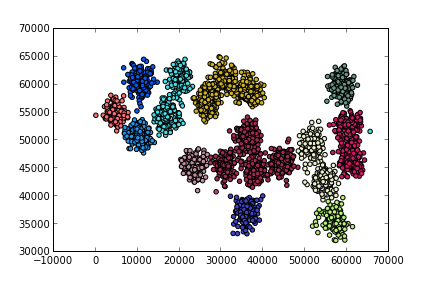
\includegraphics[height=6cm]{mstseg_01.png}

Simdi {\em SVD ile Kumeleme} yazisinda gordugumuz kelime gruplamasi ornegini
Felzenswalb ile gruplayalim. 

\begin{minted}[fontsize=\footnotesize]{python}
import scipy.linalg as lin
import scipy.sparse as sps
import itertools, sys
sys.path.append('../svdcluster/')
import leven

words = np.array(
    ['the', 'be', 'to', 'of', 'and', 'a', 'in', 'that', 'have',
     'I', 'it', 'for', 'not', 'on', 'with', 'he', 'as', 'you',
     'do', 'at', 'this', 'but', 'his', 'by', 'from', 'they', 'we',
     'say', 'her', 'she', 'or', 'an', 'will', 'my', 'one', 'all',
     'would', 'there', 'their', 'what', 'so', 'up', 'out', 'if',
     'about', 'who', 'get', 'which', 'go', 'me', 'when', 'make',
     'can', 'like', 'time', 'no', 'just', 'him', 'know', 'take',
     'people', 'into', 'year', 'your', 'good', 'some', 'could',
     'them', 'see', 'other', 'than', 'then', 'now', 'look',
     'only', 'come', 'its', 'over', 'think', 'also', 'back',
     'after', 'use', 'two', 'how', 'our', 'work', 'first', 'well',
     'way', 'even', 'new', 'want', 'because', 'any', 'these',
     'give', 'day', 'most', 'us'])

(dim,) = words.shape
f = lambda (x,y): leven.levenshtein(x,y)
res=np.fromiter(itertools.imap(f, itertools.product(words, words)),dtype=np.uint8)
A = sps.coo_matrix(np.reshape(res,(dim,dim)))
print A.shape
\end{minted}

\begin{verbatim}
(100, 100)
\end{verbatim}

Kumelemeyi yapalim, \verb!min_size=2! sectik cunku ufak kumeler de mumkun.

\begin{minted}[fontsize=\footnotesize]{python}
import felz
clf = felz.Felzenswalb(min_size=2,c=0.1)
clf.fit(A)
labels = np.array(clf.labels_)
c = len(np.unique(labels))
print c, 'clusters found'
\end{minted}

\begin{verbatim}
(100, 100)
16 clusters found
\end{verbatim}

\begin{minted}[fontsize=\footnotesize]{python}
for c in np.unique(labels):
    print 'cluster', c
    print words[labels==c]
\end{minted}

\begin{verbatim}
cluster 9
['a' 'I' 'as' 'at' 'up' 'also' 'use' 'because' 'us']
cluster 10
['in' 'it' 'with' 'which' 'its' 'first']
cluster 13
['of' 'for' 'on' 'from' 'or' 'one' 'if' 'people' 'only' 'after' 'our'
 'work']
cluster 15
['the' 'be' 'have' 'he' 'by' 'they' 'we' 'her' 'she' 'my' 'their' 'who'
 'get' 'me' 'when' 'time' 'year' 'them' 'see' 'other' 'then' 'over' 'back'
 'even' 'give']
cluster 18
['to' 'not' 'do' 'so' 'go' 'no' 'know' 'into' 'good' 'now' 'look' 'two'
 'how' 'new' 'most']
cluster 22
['this' 'his' 'him' 'think']
cluster 31
['and' 'an' 'all' 'can' 'want' 'any']
cluster 39
['that' 'what' 'than']
cluster 42
['but' 'out' 'about' 'just']
cluster 59
['make' 'like' 'take']
cluster 63
['you' 'your']
cluster 66
['would' 'could']
cluster 75
['some' 'come']
cluster 88
['will' 'well']
cluster 89
['say' 'way' 'day']
cluster 95
['there' 'these']
\end{verbatim}


Kaynaklar

[1] Pedro F. Felzenszwalb and Daniel P. Huttenlocher, {\em Efficient
  Graph-Based Image Segmentation},
\url{http://scikit-image.org/docs/dev/auto_examples/plot_segmentations.html}

[2] Bayramli B., \url{https://github.com/burakbayramli/felzenszwalb}

[3] Mihai-Cotizo Sima, {\em An extension of Felzenszwalb-Huttenlocher
  segmentation to 3D point clouds}, 2012


\end{document}
